\documentclass{article}
\usepackage{geometry}
\geometry{
    a4paper,
    left=30mm,
    right=30mm,
    top=30mm,
    bottom=30mm
}

\usepackage{annotate-equations}
\usepackage{graphicx}
\usepackage{wrapfig}
% \usepackage{figure}

\graphicspath{ {./media/} }
\usepackage[square,numbers]{natbib}
\usepackage[nottoc]{tocbibind}
\usepackage{booktabs}
\usepackage{multirow}

\usepackage{amssymb}
\usepackage{amsmath}

\usepackage{tikz}
\usepackage{listings}
\usepackage{setspace}
\definecolor{Code}{rgb}{0,0,0}
\definecolor{Decorators}{rgb}{0.5,0.5,0.5}
\definecolor{Numbers}{rgb}{0.5,0,0}
\definecolor{MatchingBrackets}{rgb}{0.25,0.5,0.5}
\definecolor{Keywords}{rgb}{0,0,1}
\definecolor{self}{rgb}{0,0,0}
\definecolor{Strings}{rgb}{0,0.63,0}
\definecolor{Comments}{rgb}{0,0.63,1}
\definecolor{Backquotes}{rgb}{0,0,0}
\definecolor{Classname}{rgb}{0,0,0}
\definecolor{FunctionName}{rgb}{0,0,0}
\definecolor{Operators}{rgb}{0,0,0}
\definecolor{Background}{rgb}{0.98,0.98,0.98}
\lstdefinelanguage{Python}{
	numbers=left,
	numberstyle=\footnotesize,
	numbersep=1em,
	xleftmargin=1em,
	framextopmargin=2em,
	framexbottommargin=2em,
	showspaces=false,
	showtabs=false,
	showstringspaces=false,
	frame=l,
	tabsize=4,
	% Basic
	basicstyle=\ttfamily\small\setstretch{1},
	backgroundcolor=\color{Background},
	% Comments
	commentstyle=\color{Comments}\slshape,
	% Strings
	stringstyle=\color{Strings},
	morecomment=[s][\color{Strings}]{"""}{"""},
	morecomment=[s][\color{Strings}]{'''}{'''},
	% keywords
	morekeywords={import,from,class,def,for,while,if,is,in,elif,else,not,and,or,print,break,continue,return,True,False,None,access,as,,del,except,exec,finally,global,import,lambda,pass,print,raise,try,assert},
	keywordstyle={\color{Keywords}\bfseries},
	% additional keywords
	morekeywords={[2]@invariant,pylab,numpy,np,scipy},
	keywordstyle={[2]\color{Decorators}\slshape},
	emph={self},
	emphstyle={\color{self}\slshape},
	%
}

\title{\textbf{Proposal for bachelor thesis}\\
Exploration of the influence of graph parameters on the generalization error of Graph Neural Networks}

\author{Author: Wensheng Zhang}

\date{\today}

\begin{document} 

\maketitle



\begin{abstract}
The goal of this bachelor thesis is to understand empirically how graph parameters/characteristics influence the generalization error of Graph Neural Networks (GNNs).
\end{abstract}


\section{Introduction}

Graph learning became a hot topic in the field of machine learning in recent years. Graph Neural Networks (GNNs) are a class of neural networks that can operate on graph-structured data. GNNs have been shown to be effective in a wide range of tasks, such as node classification, link prediction, and graph classification. However, the behavior of GNNs is not well understood. In particular, it is not clear about the relationshit between the graph parameters/characteristics and the generalization error of GNNs. The goal of this bachelor thesis is to understand empirically how graph parameters/characteristics impact the generalization error of GNNs. 

Before we untangle this problem, we need to define some terms.

In graph theory, we assume $G=(V,E)$ is an undirected graph, where $V$ is the set of nodes and $E  \subseteq \{\{v,w\}|v,w \in V , v \neq w\}$ is the set of edges. $N(v)$ is the neighborhood of a node $v$, defined as $N(v) = \{w | \{v,w\} \in E\}$. $d(v)$ is the degree of a node $v$ which refers to the number of neighbors of $v$, that is, $d(v) = |N(v)|$. 

What is a graph parameter?  A graph parameter is a function $f: \mathbb{G} \rightarrow \mathbb{R}$, which maps a graph to a real number. It characterizes a graph in a certain perspective.
For example, the average degree of the graph, the average shortest path of the graph, the centrality meature of the graph, the average number of coloring in the 1-WL algorithm, etc. I will define concrete definitions in the section \ref{sec:graph_parameters}. In my early experiment, the average degree and the average shortest path of the graph were used as graph parameters.

On the another hand, the graph classification task is a task where the goal is to classify a graph into one of several classes. In this thesis, the thesis will focus on the graph classification task. The generalization error $E_{gen}$ is a measure of how well the model generalizes to unseen data, which can be calculated as the difference between the training accuracy and the test accuracy.

Here, the accuracy $Acc$ is defined as the proportion of correctly classified graphs, that is, 
$$Acc = \frac{\text{Number of correctly classified graphs}}{\text{Total number of data points}}$$

The generalization error is defined as
\\

\begin{equation*}
    E_{gen} = \eqnmarkbox[blue]{node1}{Acc_{train}} - \eqnmarkbox[blue]{node2}{Acc_{test}}
\end{equation*}
\annotate[yshift=0.5em]{left}{node1}{over train dataset}
\annotate[yshift=0.5em]{right}{node2}{over test dataset}

Why is it important to understand the influence of graph parameters on the generalization error of GNNs? The understanding of the influence of graph parameters on the generalization error of GNNs can help us to understand the behavior of GNNs so that researchers can can tune GNNs to improve their predictive performance on new graphs.
\section{Setup in the early experiment}
In following, I will descripe training framework, datasets, models and concrete graph parameters for the setup of the experiment.

\subsection{Training Framework}
The training framework is based on PyTorch Geometric~\cite{fey2019fast}. PyTorch Geometric is a library for deep learning on graphs and other irregular structures. It consists of various methods and utilities to ease the implementation of GNNs. 

\subsection{Datasets}
The dataset used for the classification is TUDataset~\cite{morris_tudataset_2020}. TUDataset is often used for the GNN evaluation. It consists of data from different domains, including small molecules, bioinformatics, social networks and synthetic. Since the size of some datasets is quiet small (less than 500 data points/graphs), I use 10-fold cross validation in the training process, in order to fully utilize the data. A dataset is split into 1:1:8, where one of the folds is treated as the test dataset and another is treated as the validation dataset. The remaining folds are used for training. 

In the early experiment, I took 10 datasets from different domains as examples. The datasets are Mutagenicity, NCI1, COIL-RAG, Letter-high, DD, PROTEIN\_full, COLORS-3, AIDS, ENZYMES, Cuneiform. In the future, I will explore more datasets in the experiment.

\subsection{Models}
In the early experiment, I have used Graph Convolutional Networks(GCN) layer~\cite{kipf2017semisupervised} and Graph Attention Networks(GAT) layer~\cite{velickovic2020pointer} to construct models. In order to overfitting, dropout is used in the model and Relu function is used as activation function. In the Appendix, I have provided the code of example models. In the future, I will explore more GNN layers in the experiment, including Simplified Graph Convolution(SGC)~\cite{wu2019simplifying}, GATv2~\cite{brody2021attentive} and Message Passing Neural Networks(MPNN)~\cite{gilmer2017neural} etc.


\subsection{Graph Parameters Unter Investigation} \label{sec:graph_parameters}
As graph parameters defined abstractly above, I give here the concrete definition of the graph parameters in the experiment.\\
\begin{description}
    \item [Average degree] The average degree of the graph $d_{avg}$ is defined as the average of the degrees of all nodes in the graph, that is
    $$ d_{avg} = \frac{1}{|V|} \sum_{v \in V} d(v)$$
    \item [Average shortest path length] The average shortest path length of the graph $a$ is defined as the average of the shortest paths between all pairs of nodes in the graph. The shortest path $d(s, t)$ between two nodes $v$ and $w$ is the minimum number of edges that need to be traversed to go from $v$ to $w$. The formal definition is
    $$
a = \frac{1}{|V|(|V|-1)} \sum_{v \in V} \sum_{w \in V, w \neq v} d(v, w)
    $$
    \item [Centrality measure of graphs] At first we have the definition of centrality measure in the \textbf{node level}. The centrality measure of a node is a measure of the importance of the node in the graph. There are many centrality measures, such as degree centrality, closeness centrality, betweenness centrality, and eigenvector centrality. 
    
    \textit{Degree centrality} is identical to the average degree of the graph defined above. 
    
    \textit{Closeness centrality} $C_C(v)$ is defined as the reciprocal of the sum of the length of shortest paths from the node $v$ to all other nodes in the graph, that is 
    $$C_C(v) = \frac{1}{\sum_{w\in V}{d(v ,w)}}$$
    where $d(v, w)$ is the shortest path between node $v$ and node $w$. 
    
    \textit{Betweenness centrality} $C_B(v)$ is the sum of the fraction of all-pairs shortest paths that pass through $v$. The definition can be given by the expression:
    $$
        C_B(v) = \sum_{s,t \in V} \frac{\sigma_{st}(v)}{\sigma_{st}}
    $$
    where $\sigma_{st}$ is the number of shortest paths between nodes $s$ and $t$, and $\sigma_{st}(v)$ is the number of shortest paths between nodes $s$ and $t$ that pass through node $v$.
    
    \textit{Eigenvector centrality} Eigenvector centrality is a measure of the influence of a node in a graph based on the concept that connections to high-scoring nodes contribute more to the score of the node in question. Formally, the eigenvector centrality $C_E(v)$ of a node $v$  is defined as the $v$ -th component of the eigenvector corresponding to the largest eigenvalue of the adjacency matrix $A$ of the graph. Mathematically, it can be expressed as:
    
    \[ C_E(v) = \frac{1}{\lambda} \sum_{u \in N(v)} a_{vu} C_E(u) \]
    
    where $ \lambda$ is the largest eigenvalue of the adjacency matrix $A$.
$a_{vu}$ is the element of the adjacency matrix $A$ corresponding to the edge between nodes $v$  and $u$.
$ C_E(u)$  is the eigenvector centrality of node $u$.


    Finally in the \textbf{graph level}, the centrality measure of the graph is defined as the average of the centrality measures over all nodes in the graph.
    \item [Average number of coloring in the 1-WL algorithm] The 1-dimensional Weisfeiler-Leman algorithm (1-WL) is a algorithm that assigns a unique label(color) to each node in the graph. The average number of coloring in the 1-WL algorithm is defined as the average number of colors used to color the nodes in the graph. The 1-WL algorithm is a powerful graph isomorphism algorithm that can be used to determine if two graphs are isomorphic. I give the procedure of the 1-WL algorithm here:
    \begin{enumerate}
        \item Assign the same color to all nodes in the graph.
        \item Two nodes $v$, $u$ are assigned a different color if there is a color c such that the number of c-colored neighbors of $u$ is not equal to the number of c-colored neighbors of $v$.
        \item Repeat step 2 until the colors of all nodes do not change.
    \end{enumerate}
    
\end{description}


Besides the graph parameters defined above, I will explore more graph parameters in the experiment if possible.

\section{Experiment}
% 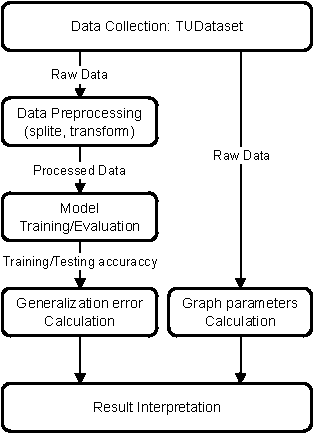
\includegraphics{experiment_procedure.pdf}


\begin{figure}[h]
    \centering
    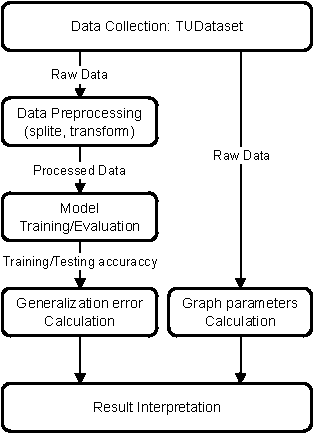
\includegraphics[width=0.5\textwidth]{experiment_procedure.pdf}
    \caption{A illutration of experiment Procedure}
    \label{fig:experiment}
\end{figure}

The experiment consists in three parts: 1. Train the models from datasets and evaluate the models to calculate the generalization error. 2. calculate the parameters of the graphs from the dataset. 3. Analyze the influence of the graph parameters on the generalization error of the GNNs. (See Figure~\ref{fig:experiment})


\subsection{Experimental details in the early stage}
Initially, I use Adam optimizer with learning rate 0.01. The batch size is set to 64. The hidden dimension of the GNN layer is set to 64. The number of epochs is set to 200. To prevent overfitting and to save time, the early stopping is used with patience 20. The loss function is set to CrossEntropyLoss. 

In the future, I will explore different hyperparameters, such as learning rate, batch size, size of hidden dimension, and patience in the early stopping.

% \clearpage


\section{Results of early experiment} \label{sec:results}

Here I take ten datasets from TUDataset as examples. The calculated parameters are shown in Table~\ref{tab:parameter}. The generalization error of the models are shown in Table~\ref{tab:error}. 


\begin{table}[h!]
    \centering
    \begin{tabular}{@{}lll@{}}
    \toprule
    \multicolumn{1}{c}{\multirow{2}{*}{Dataset}} & \multicolumn{2}{c}{Parameter}                                            \\ \cmidrule(l){2-3} 
    \multicolumn{1}{c}{}                         & \multicolumn{1}{c}{Ave. degree} & \multicolumn{1}{c}{Ave. shortest path} \\ \midrule
    Mutagenicity                                 & 2.0379         & 4.4825                     \\
    NCI1                                         & 2.1550         & 5.4697                     \\
    COIL-RAG                                     & 1.8277         & 1.0606                     \\
    Letter-high                                  & 1.8896         & 1.5173                     \\
    DD                                           & 4.9790         & 7.9700                     \\
    PTOTEIN\_full                                & 3.7346         & 4.7123                     \\
    COLORS-3                                     & 2.9288         & 2.0945                     \\ 

    AIDS  &  2.01286  & 3.2864 \\
    ENZYMES  &  3.8626  & 4.4461 \\
    Cuneiform  &  4.0795  & 2.24442 \\ \bottomrule

    \end{tabular}
    \caption{The calculated parameters from a set of datasets, here used two parameters, the average degree of the graph and the average shortest path of the graph which defined in the section \ref{sec:graph_parameters}.}
    \label{tab:parameter}
\end{table}

\begin{table}[h!]
    \centering
    \begin{tabular}{@{}lll@{}}
    \toprule
    Dataset        & Ave. generalization error & Standard Deviation   \\ \midrule
    Mutagenicity   & 0.0268      & 0.02335 \\
    NCI1           & 0.0138      & 0.02649 \\
    COIL-RAG       & 0.0450      & 0.01378 \\
    Letter-high    & 0.0403      & 0.04342 \\
    DD             & 0.0524      & 0.05849 \\
    PROTEINS\_full & 0.0189      & 0.05032 \\
    COLORS-3       & 0.0076      & 0.01428 \\
    AIDS           &  0.00931    & 0.008642 \\
    ENZYMES           &  0.0345    & 0.052339 \\
    Cuneiform           &  0.2392    & 0.09868 \\ \bottomrule
    \end{tabular}
    \caption{The table shows the calculated generalization error from a set of datasets, where the generalization error is calculated as the difference between the training accuracy and the test accuracy.}
    \label{tab:error}
\end{table}



I then used a scatter plot to visualize the generalization error against the two graph parameters. The result is shown in Figure~\ref{fig:scatter}. Also I calculated the correlation between the generalization error and the graph parameters. The result is shown in Table~\ref{tab:correlation}.

\begin{figure}[h!]
    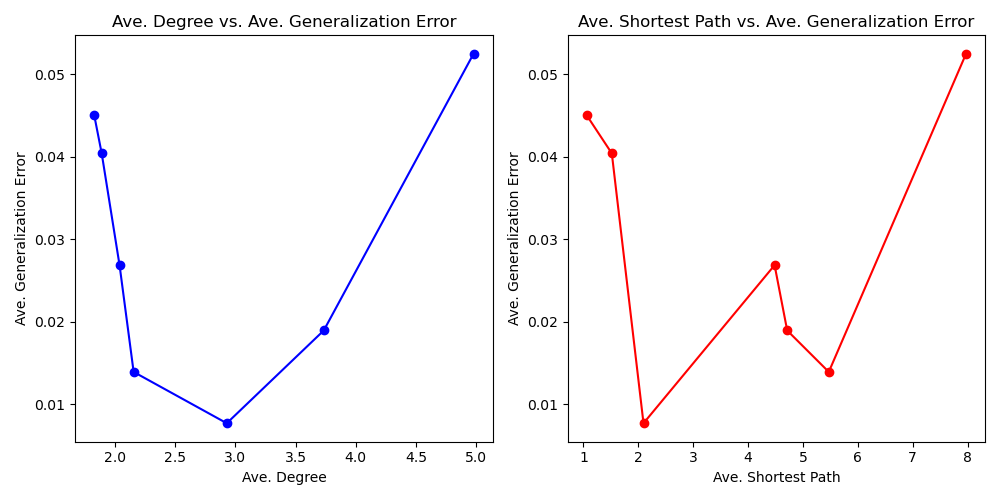
\includegraphics[width=\textwidth]{final_results.png}
    \caption{The generalization error against the graph parameters, the x-axis is the average degree of the graph, the y-axis is the generalization error of the model. The each point in the plot is the calculated result from different datasets. It is obvious that more datasets are needed to get more reliable results.}
    \label{fig:scatter}
\end{figure}


\begin{table}[h]
    \centering
    \begin{tabular}{@{}ll@{}}
    \toprule
                       & Ave. Generalization Error \\ \midrule
    Ave degree            & 0.4068                    \\
    Ave. shortest path & -0.2074                   \\ \bottomrule
    \end{tabular}
    \caption{The correlation between the generalization error and the graph parameters. The correlation is calculated by the Pearson correlation coefficient.}
    \label{tab:correlation}
    \end{table}

\newpage

\section{Objective of the thesis}

The Objective of this bachelor thesis is to understand empirically how graph parameters/characteristics influence the generalization error of GNNs. Beside the content of early experiment, I will explore more GNN layers in the experiment, such as Simplified Graph Convolution(SGC)~\cite{wu2019simplifying}, GATv2~\cite{brody2021attentive} and Message Passing Neural Networks(MPNN)~\cite{gilmer2017neural} etc.
I will explore all the graph parameter I mensioned in \ref{sec:graph_parameters} and more if possibly. 

I will also explore different hyperparameters, such as learning rate, batch size, hidden dimension, number of epochs, and patience in the early stopping to find the best setting for the models/datasets. 


In the section~\ref{sec:results}, I have made the experiment on 10 datasets. In the future, I will make the experiment on more datasets to get more reliable results.

\clearpage

\tableofcontents

\newpage

\bibliographystyle{abbrvnat}
\bibliography{main} % refers to example.bib

% All reduce Graphs
\newpage 

\section{Appendix} 
 
\subsection*{Example of GCN model}

\begin{lstlisting}[language=Python]
import torch
from torch import nn
import torch.nn.functional as F
from torch_geometric.nn import GCNConv
from torch_geometric.nn import global_mean_pool


class GCN(torch.nn.Module):
    def __init__(self, in_channels, hidden_channels, out_channels):
        super().__init__()
        self.conv1 = GCNConv(in_channels, hidden_channels)
        self.conv2 = GCNConv(hidden_channels, hidden_channels)
        self.conv3 = GCNConv(hidden_channels, hidden_channels)
        self.conv4 = GCNConv(hidden_channels, hidden_channels)
        self.fc1 = nn.Linear(hidden_channels, hidden_channels)
        self.fc2 = nn.Linear(hidden_channels, out_channels)


    def forward(self, x, edge_index, batch, edge_weight=None):
        x = self.conv1(x, edge_index, edge_weight).relu()
        x = self.conv2(x, edge_index, edge_weight).relu()
        x = self.conv3(x, edge_index, edge_weight).relu()
        x = self.conv4(x, edge_index, edge_weight).relu()
        x = global_mean_pool(x, batch)
        x = self.fc1(x).relu()
        x = F.dropout(x, p=0.5, training=self.training)
        x = self.fc2(x)
        return x
    
    def reset_parameters(self):
        for (_, module) in self._modules.items():
            module.reset_parameters()

\end{lstlisting}

\end{document}